\documentclass{article}
\usepackage{times}
\usepackage{helvet}
\usepackage{courier}
\frenchspacing
\setlength{\pdfpagewidth}{8.5in}
\setlength{\pdfpageheight}{11in}
\usepackage{float}
\usepackage[letterpaper, margin=1in]{geometry}
% for displaying code
\usepackage{listings}

\usepackage{hyperref}
\hypersetup{plainpages=false,
	breaklinks=true,
    colorlinks=true,
    urlcolor=blue,
    citecolor=blue,                                       
    linkcolor=blue,
    bookmarksopen=true,
    bookmarksdepth=3,
    bookmarksopenlevel=3,
    pdfstartview=FitV,
    pdfdisplaydoctitle=true}

\usepackage[american]{babel}
\usepackage[backend=biber,natbib=true,style=apa,citestyle=authoryear,giveninits=true,uniquename=false,useprefix=true,apamaxprtauth=99,maxbibnames=99,sorting=nyt]{biblatex}
\DeclareLanguageMapping{american}{american-apa}
\addbibresource{Mendeley.bib}

\usepackage[utf8]{inputenc}
\usepackage{csquotes}
\usepackage{amsmath}
\usepackage{amsthm}
\usepackage{amsfonts}
\usepackage{graphicx}
\usepackage[colorinlistoftodos]{todonotes}
\usepackage{afterpage}
\usepackage{comment}
\usepackage{algorithm}
\usepackage{algorithmicx}
\usepackage{algpseudocode}
\usepackage{float}

\pdfinfo{
/Title (CMPUT 652, Fall 2019 - Assignment #2)
/Author (Craig Sherstan)
/Keywords ()}
 
\DeclareGraphicsExtensions{.pdf, .png, .jpg}
 
\newcommand{\x}{{\bf x}}
\newcommand{\X}{{\bf X}}
\newcommand{\bv}{{\bf v}}
\newcommand{\y}{{\bf y}}
\newcommand{\w}{{\bf w}}
\newcommand{\PI}{{\bf \Pi}}
\newcommand{\Real}{{\mathbb{R}}}
\newcommand{\q}{{\bf q}}
\newcommand{\br}{{\bf r}}
\newcommand{\bP}{{\bf P}}
\newcommand{\D}{{\bf D}}
\newcommand{\A}{{\bf A}}
\newcommand{\bb}{{\bf b}}
\newcommand{\I}{{\bf I}}
\newcommand{\on}{\operatorname}
\newcommand{\E}{\on{E} }

% Dankness incoming
% Box environment for adding visible notes work-in-progress
\usepackage{mdframed}
\newenvironment{todobox}[1][]{%
\ifstrempty{#1}%
{\mdfsetup{%
frametitle={%
\tikz[baseline=(current bounding box.east),outer sep=0pt]
\node[anchor=east,rectangle,fill=red!20]
{\strut TODO};}}
}%
{\mdfsetup{%
frametitle={%
\tikz[baseline=(current bounding box.east),outer sep=0pt]
\node[anchor=east,rectangle,fill=red!30]
{\strut TODO: ~#1};}}%
}%
\mdfsetup{innertopmargin=10pt,linecolor=red!70,%
linewidth=2pt,topline=true,%
frametitleaboveskip=\dimexpr-\ht\strutbox\relax
}
\begin{mdframed}[]\relax}{\end{mdframed}}
%%\end{dankness}

\title{CMPUT 652, Fall 2019 - Assignment \#2}
\date{October 15, 2019}
% \author{Craig Sherstan}

\begin{document}
\maketitle

\begin{center}
    Version: 1.1. October 16, 2019.
\end{center}

\begin{tabular}{c c}
     \textbf{Due}: & October 29, 23:59 MST \\
\end{tabular}\\

This assignment consists of two parts. The first are written questions which are related to the course lectures. The second part is a programming assignment. You will need to submit both code and a write up. Please provide these as a single archive. Submit to both armahmood@ualberta.ca and sherstan@ualberta.ca.

\newcommand{\imgheight}{2.0in}

\section{Written Questions}
Total 30 points. Complete  within the given space using \LaTeX ~or handwritten notes. Show the derivations or the steps for obtaining partial points. On the other hand, mistakes, missteps or bad reasoning behind a correct answer will result in points deducted.

\newpage

\subsection{\normalsize 
Consider a finite MDP, where a state is represented by a $d$-dimensional feature vector $\x(s)$, and the feature vectors for all $N$ states form a $N\times d$ feature matrix $\X$ with rank $d$. 
The Mean Squared Value Error (MSVE) objective is $\Vert \bv_\pi - \X\w \Vert^2_{\D_\pi}$, where $\bv_\pi$ is an $N$-dimensional vector, $[\bv_\pi]_s = v_\pi(s)$ is the value of state $s$ induced by policy $\pi$, and $\D_\pi$ is a $N\times N$ diagonal matrix with the steady-state probabilities $d_\pi(s)$ induced by $\pi$ along the diagonal. Show that the solution to this objective is $\w^*_{\on{VE}} = (\A_{\on{VE}})^{-1} \bb_{\on{VE}}$, where $\A_{\on{VE}} = \X^\top \D_\pi\X$ and $\bb_{\on{VE}} = \X^\top\D_\pi \bv_\pi$
 (15 points).
}


\begin{align*}
	\Vert \bv_\pi - \X\w \Vert^2_{\D_\pi} &= (\bv_\pi - \X\w)^\top \D_\pi (\bv_\pi - \X\w) \\
	&= \bv_\pi^\top \D_\pi \bv_\pi - \w^\top\X^\top\D_\pi\bv_\pi - \bv_\pi^\top\D_\pi\X\w + \w^\top\X^\top\D_\pi\X\w \\
	\\
	\nabla_\w \Vert \bv_\pi - \X\w \Vert^2_{\D_\pi} &= -2\X^\top\D_\pi\bv_\pi + 2\X^\top\D_\pi\X\w = 0\\
	&\rightarrow \X^\top\D_\pi\X\w = \X^\top\D_\pi\bv_\pi \\
	&\rightarrow \w^*_{\on{VE}} = (\X^\top\D_\pi\X)^{-1}\X^\top\D_\pi\bv_\pi\\
	&\text{The inverse is valid here because $ \X, \D_\pi $ are both full-rank matrices}\\
	&\rightarrow \w^*_{\on{VE}} = (\A_{\on{VE}})^{-1} \bb_{\on{VE}}
\end{align*}


\newpage

\subsection{\normalsize 
Consider a vector $\y$ that may not be in the linear span of the features, that is, $\y\ne\X\w$ for any $\w\in\Real^d$. The projection matrix $\PI$ is such that $\PI \y = \X\w_y $, where $\w_y = \arg\min_{\w} \Vert \y - \X\w \Vert^2_\D$, that is, it is the matrix that linearly transforms or ``projects'' $\y$ to the span of features according to norm $\Vert \cdot \Vert^2_\D$. Here $\D$ is a diagonal matrix with positive diagonal elements. Show that $\PI = \X(\X^\top \D\X)^{-1}\X^\top\D$, $\PI\X=\X$ and $\X^\top\D\PI=\X^\top\D$
 (15 points).
}

\begin{align*}
	&\hspace{-20px}\text{Based on the answer for Q1.1, we know: } \\
	\w_y &= (\X^\top\D_\pi\X)^{-1}\X^\top\D_\pi y \\
	\\
	\PI \y &= \X\w_y\\
	&= \X(\X^\top\D\X)^{-1}\X^\top\D y \\
	&\rightarrow \PI = \X(\X^\top \D\X)^{-1}\X^\top\D\\
	\\
	\PI\X &= \X(\X^\top \D\X)^{-1}\X^\top\D \X\\
	&= \X(\X^\top \D\X)^{-1}(\X^\top\D \X) \\
	&= \X \\
	\\
	\X^\top\D\PI &= \X^\top\D \X(\X^\top \D\X)^{-1}\X^\top\D \\
	&= (\X^\top\D \X)(\X^\top \D\X)^{-1}\X^\top\D \\
	&= \X^\top\D
\end{align*}


\newpage

\section{Programming}
\label{sec:programming}

100 points. You will implement a basic policy-gradient method: REINFORCE with a Baseline. The purpose is to gain experience implementing PG methods in PyTorch. Additionally, the questions are meant to help you develop the tools you will need for performing empirical analysis.

See Sections 13.3 and 13.4 of \fullcite{Sutton2018} for information on the REINFORCE algorithm.

\begin{figure}[h]
\begin{center}
\centerline{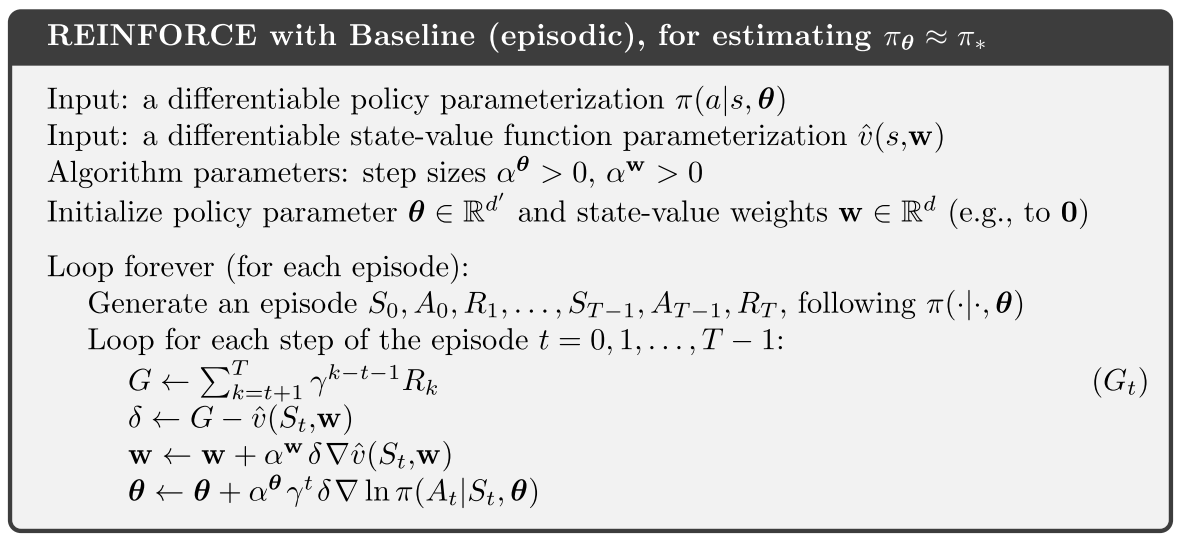
\includegraphics[height=\imgheight]{img/REINFORCE.png}}
\caption{\citep{Sutton2018}}
\label{fig:reinforce}
\end{center}
\end{figure}

The episodic REINFORCE algorithm collects entire episodes of trajectories before updating policy parameters. It is a Monte Carlo method based on Stochastic Gradient Descent. In the  its returns can have high variance, making learning difficult. By subtracting off a baseline, the value estimate, the variance of the policy parameter updates can be reduced and learning can be improved.

Your task is to implement REINFORCE with a baseline to solve the classic Cart Pole task: \url{https://gym.openai.com/envs/CartPole-v1/}.

Note that the algorithm specified in the above collects an episode of transitions and then loops over each transition of the episode computing gradients and updating weights at each timestep. You could also implement the update as a batch where the errors are taken across the entire episode trajectory before gradients are computed. Feel free to implement either approach. However, for reporting losses please average losses over the whole episode.

A note on $\gamma$. First, $\gamma$ is sometimes approached in two different ways. One way claims that $\gamma$ is part of the problem definition and the other treats $\gamma$ as part of the solution. We will take the second view here. We will evaluate your algorithm based on the total undiscounted reward received over an entire episode. You are free to adjust $\gamma$ as you need, but a good place to start would be to simply set $\gamma=1$ and then try other values. Further, the last line of the equation in Figure 1 has the additional term $\gamma^t$. This term was not always included in the algorithm and you will find implementations online which leave out this term. I expect it will impact the values of $\gamma$ for which your algorithm performs well. You are free to include it or leave it out, but you should be clear which version you implemented in your pseudocode.

\subsection{Setup}

Create a python virtualenv (feel free to use another dependency manager if you like) for running your code. We will use python3.6+. A requirements.txt file is included specifying all the packages which you will require for your virtualenv. Do not make your code dependent on any additional packages as they will not be part of the environment on which I test.

Create your virtualenv as follows (adjust paths as required):

\begin{verbatim}
    # create a virtualenv called assign2
    virtualenv --python=python3.6 assign2
    # you will need to activate this environment before running your script.
    source assign2/bin/activate
    pip install -r requirements.txt
\end{verbatim}

You have been provided with two skeleton files: main.py and network.py. Edit these files to implement your code.

\subsection{Deliverables}

Note, that I am not evaluating your code based on whether or not it can beat some baseline or the performance of your classmate's algorithm. I am looking for code that works. Your agent should be able to fairly frequently achieve a perfect score of 200 by at least 10k episodes. I will be lenient in grading, but I do expect that everyone put in the effort and does their own work - of course you are free to consult with one another. The key to full marks is to simply implement the algorithm, achieve reasonable performance, and put in sufficient effort in answering the questions and formatting your plots where possible. If everything looks good from a high level, I won't go looking for problems.

The plots provided below should only be taken as examples, not optimal.

In the following code we have chosen to plot returns as a function of the episode. We do this for simplicity. A fairer comparison would be to compare based on the number of observations made. In the next assignment we will compare in this way.

\subsubsection{Running Code (50 points)}

\begin{figure}[H]
\begin{center}
\centerline{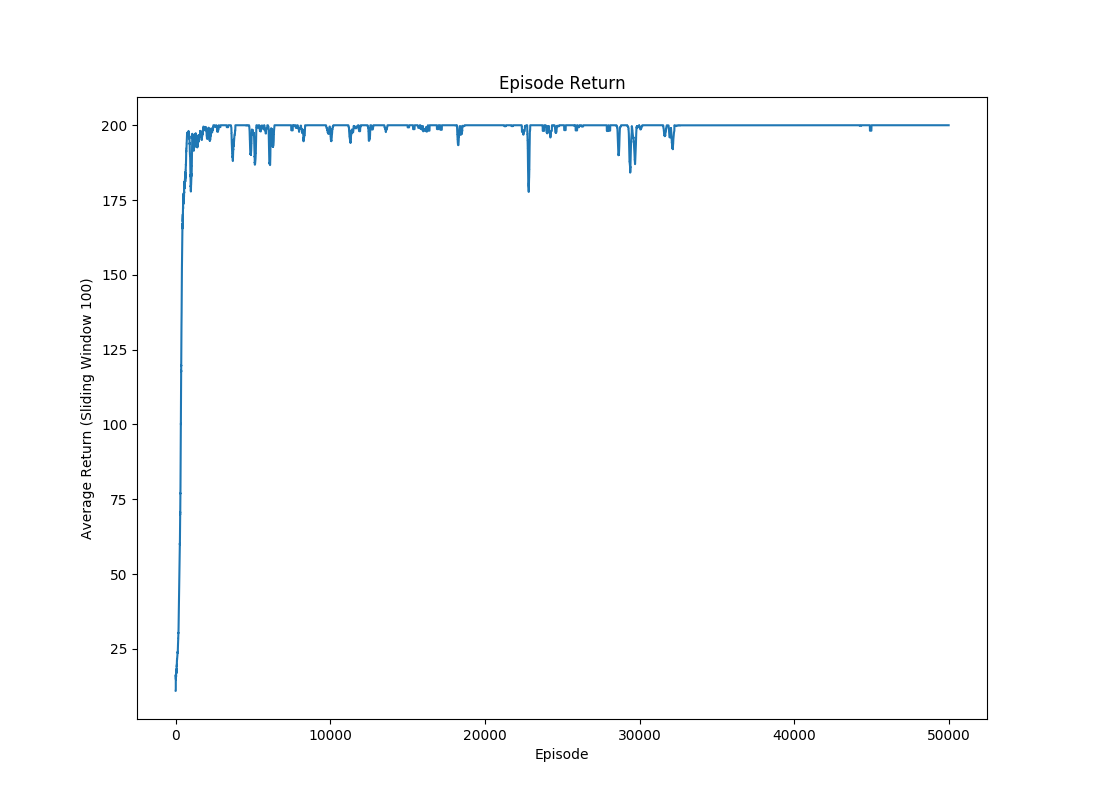
\includegraphics[scale=0.5]{img/my_return.png}}
\end{center}
\end{figure}


\begin{algorithm}[H]
	\caption{REINFORCE with Baseline}
	\begin{algorithmic}
		\Require Initialize policy network $ \pi(A|S, \theta) $ and value network $ v(S|w) $
		\For {$episode = 1, M$}
			\State Generate an episode $ S_0, A_0, R_1, \cdots, S_{T-1}, A_{T-1}, R_T $ with policy $ \pi(\cdot|\cdot, \theta) $
			\For {each step of the episode $ t=0,1,\cdots, T-1 $}
			\State $G_t \leftarrow\sum^T_{k=t+1}\gamma^{k-t-1}R_k$
			\State $\delta \leftarrow G_t - v(S_t, w) $
			\State $ w \leftarrow \alpha \delta \nabla v(S_t, w) $
			\State $ \theta \leftarrow \alpha \delta \nabla \ln\pi(A_t|S_t,\theta) $
			\EndFor
		\EndFor
	\end{algorithmic}
\end{algorithm}


\subsubsection{Saved Policy (5 points)}

See "saved.pkl", load it by "python3 main.py -l"

\subsubsection{Plot Return vs. Episode (15 points)}

Perform 30 different runs for your algorithm (each run should be a different random initialization). Each run should be 5000 episodes in length. For each run you will need to save the list of episode returns. Using this data you will produce two different plots looking at the mean performance across different runs. Plots should be labeled and legible - they should look nice and be something you would include in a paper submission.

\begin{enumerate}
    \item From your data set sample 3 runs and take the mean across the runs. Do this 10 times, each time resampling from your set of 30 runs. Plot each of these means together on a single plot. To be clear the x-axis will be the episode number.
    
    \begin{figure}[H]
    	\begin{center}
    		\centerline{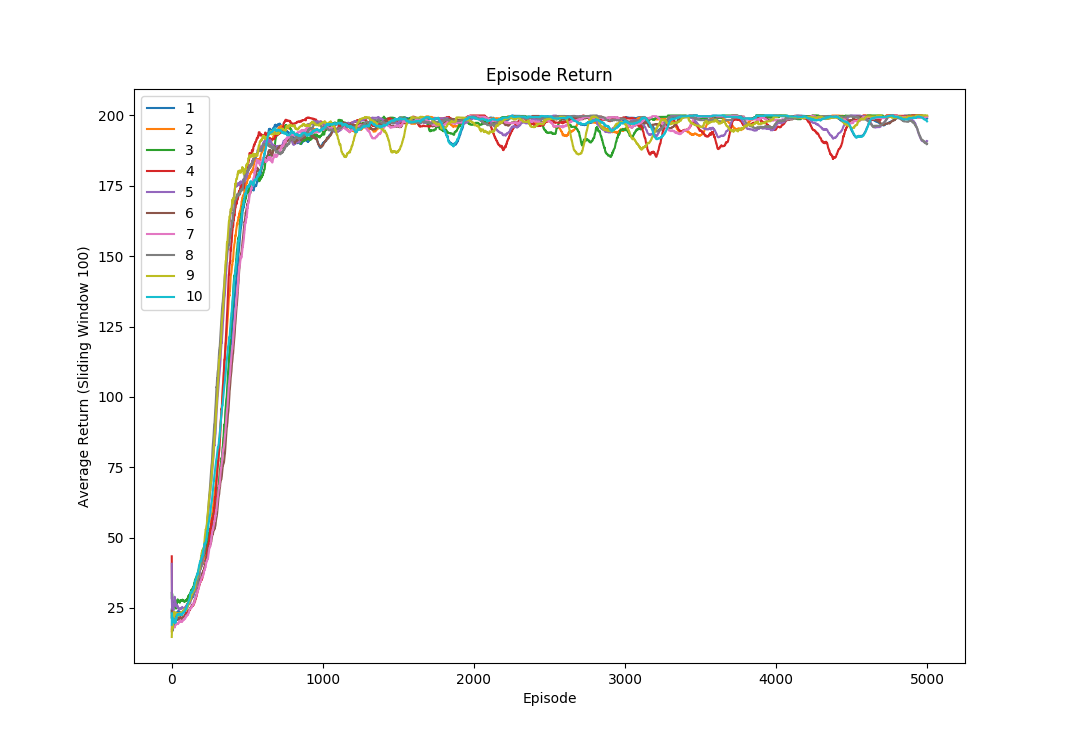
\includegraphics[scale=0.5]{img/mixture_of_mean.png}}
    	\end{center}
    \end{figure}
    
    \item From your dataset plot means for the following: 3 runs, 10 runs, 30 runs. Plot these all on the same plot. Label the lines in some way.
    
    \begin{figure}[H]
    	\begin{center}
    		\centerline{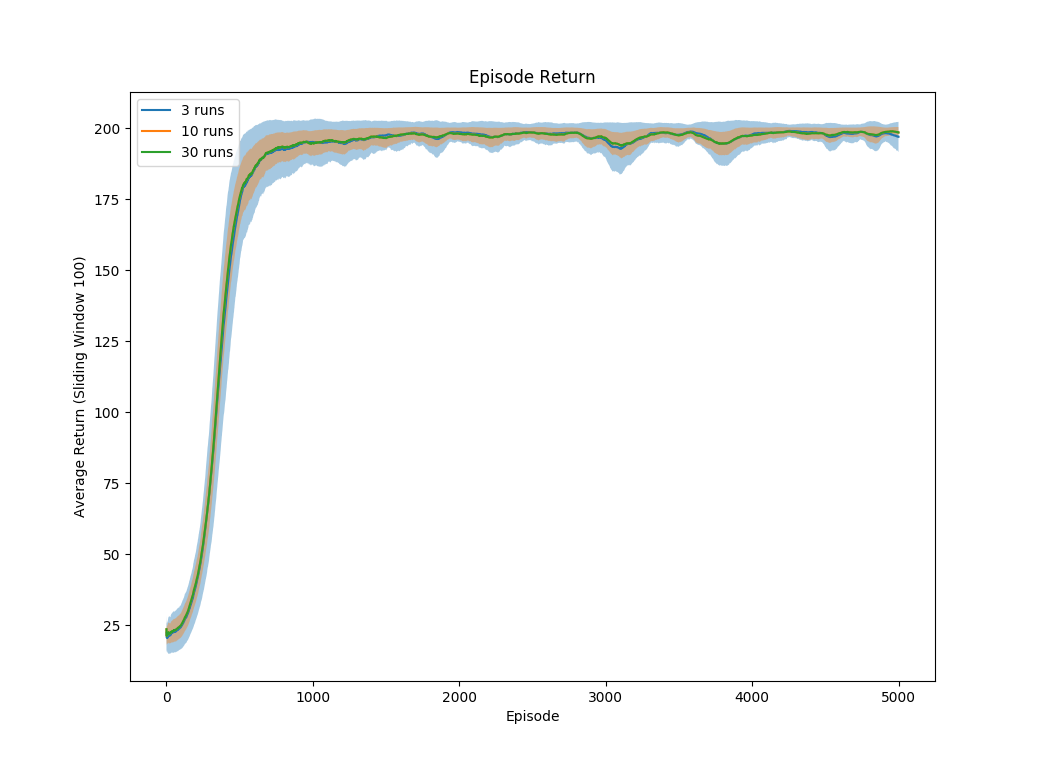
\includegraphics[scale=0.5]{img/mean_with_std.png}}
    	\end{center}
    \end{figure}
        
\end{enumerate}

\noindent\textbf{Question:} There are different statistics which might be reported for each mean: standard deviation, max-min, standard error. Which of these would you use? When? Why? In the previous plot which would you use to give a comparison between the series? Include your answer to these questions. 

I would use standard deviation to compare between the previous results once the learning curves converge. Standard deviation is used here because it's an appropriate statistic for possible deviation from the expected value within certain confidence interval. Max-min is not used here because it's extremely sensitive to outliers and contains no information about confidence interval. Standard error is not used as in reinforcement learning, we usually have limited number of returns whose standard deviation can be explicitly computed instead of estimating with standard error.




\subsubsection{Algorithm Comparison: (15 points)}

In this question, I compared the performance of REINFORCE with or without the term $ \gamma^t $ in the policy update $ \w \leftarrow{} \w + \alpha^{\w}\gamma^t \delta \nabla \text{ln} \pi(A_t|S_t,\w) $. In my previous implementation, I didn't include this term as current algorithms usually ignore this term. The figure given below is the mean and standard deviation of 30 run with random initialization.

\begin{figure}[H]
	\begin{center}
		\centerline{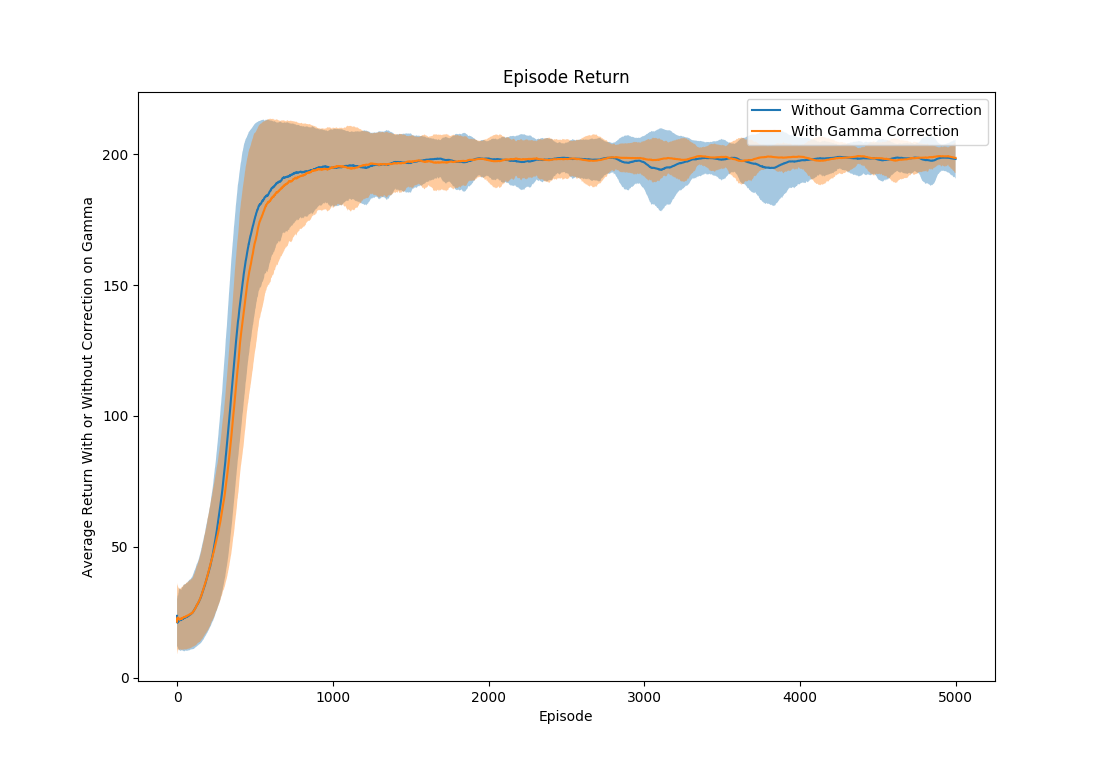
\includegraphics[scale=0.5]{img/gamma.png}}
	\end{center}
\end{figure}

In first roughly 800 episode, where the episode return is rapidly increasing, update without the $ \gamma^t $ term learns slightly faster than the other one, but they have similar standard deviation in performance. My explanation here is that adding the $ \gamma^t $ term has the effect of making smaller steps in gradient update in general which resulted in slower learning.

However, when both methods converge, method with the $ \gamma^t $ term has noticeable lower variance and the performance curve is also more flatten than the other one. I think this is also because of the smaller steps in gradient update by $ \gamma^t $. Making gradient update with a large step size is likely to degrade current policy, especially when current policy is near-optimal. Such a problem is addressed in methods like TRPO or PPO, but using smaller learning rate could yield the similar effect to some extent.


\subsubsection{Tensorboard file: (15 points)}

See "./runs"


\subsection{Submission Checklist}


\begin{itemize}
    \item[$\square$] \hspace{-15px} $\checkmark$ \textbf{2.2.1} Source Code and output plot from one run. Written algorithm.
    \item[$\square$] \hspace{-15px} $\checkmark$
    \textbf{2.2.2} One saved policy.
    \item[$\square$] \hspace{-15px} $\checkmark$
    \textbf{2.2.3} Two plots and 1 answered question.
    \item[$\square$] \hspace{-15px} $\checkmark$
    \textbf{2.2.4} A short writeup of your comparison. One plot showing the comparison.
    \item[$\square$] \hspace{-15px} $\checkmark$
    \textbf{2.2.5} One TensorBoard events file.
\end{itemize}

\subsection{Common Problems to Watch For}

\begin{itemize}
    \item Forgetting to link your optimizer with your policy parameters.
    \begin{verbatim}
        torch.optim.Adam(network.parameters())
    \end{verbatim}
    \item Forgetting to \verb|zero_grad| before calling \verb|backward|.
    \item Broadcasting issues. If two vectors of different sizes are attempted to combine, e.g. [26] and [26,1], torch and numpy may happily combine these, but the results may not be what you expect. This can give incorrect results.
    \item Wrapping data in \verb|torch.Tensor()| breaks the gradient flow. For example, if you want to convert a list of tensors to a tensor use \verb|torch.stack()| instead.
    \item Forgetting to call \verb|detach()| on a bootstrapped target. You don't, usually, want the gradient taken through your target. When we use a bootstrapped target, like in TD learning, we need to make sure to detach the gradient through the target.
\end{itemize}

\end{document}